
\chapter{图像处理基本理论}

\section{图像增强}

实际图像不是完美的。由于噪声和光照等原因\upcite{imgproc},图像的质量达不到自动识别的要求,所以需要进行图像增强。图像增强可以突出待识别的目标的特征,抑制噪声和目标外的部分,从而使增强的图像更适合计算机识别。常见的图像增强方法有\emph{灰度变换}和\emph{图像平滑}\upcite{compvision}。

\subsection{灰度变换}

灰度变换就是将图像每个像素的灰度变换成另一种灰度。灰度变换后每个像素的灰度仅仅由变换前的灰度决定。如果输入图像为$F(i,j)$,输出图像为$G(i,j)$,则灰度变换可以表示为\upcite{imgproc}:
\begin{equation}
  G(i,j)=T(F(i,j))
\end{equation}
变换函数$T(x)$可以由用户指定,也可以根据直方图确定。\emph{直方图均衡}就是一种根据直方图确定变换函数的方法。直方图均衡主要用于增加图像的全局对比度,改善光照条件不佳的图像。例如对背景或前景过亮或过暗的图像进行光照补偿,增强曝光过度或曝光不足的图像的细节等。直方图均衡化使输出图像包括所有可能的灰度级,并在每个灰度级上有大致相等的像素个数。要达到上述要求,首先求出直方图。设$n$表示图像的像素数,$n_i$表示灰度$i$出现的次数。灰度$i$有$0,1,\cdots,L-1$共$L$个灰度级。则直方图均衡化的灰度变换函数$T(x)$可以用如下方式求出。直方图$p(i)$表示灰度$i$出现的概率,用公式表示为\upcite{otsu}:
\begin{equation}
  \label{eq:hist}
  p(i)=\frac{n_i}{n},i=0,1,\cdots,L-1
\end{equation}
再从直方图求出累计概率函数$c(i)$,定义如下:
\begin{equation}
  \label{eq:acc}
  c(i)=\sum_{j=0}^i p(j)
\end{equation}
最后将$c(i)$映射到$L$个灰度级\upcite{opencvref}:
\begin{equation}
  \label{eq:map}
  m(c(i))=\left[\frac{c(i)-\min(c(i))}{\max(c(i))-\min(c(i))}\cdot L\right]
\end{equation}
此时得到灰度变换函数为$T(x)=m(c(x))$。

\subsection{平滑滤波}

原始图像一般含有较多的噪声。噪声一般表现为盐椒噪声或孤立的点线噪声。图像平滑滤波使图像模糊化,去除极小的细节或将图像内的小间断连接起来。图像平滑滤波的基本方法是在像素的邻域内,对邻域内的像素和对应的系数的乘积求和\upcite{imgproc}。邻域内像素位置对应的权值一般用\emph{模板}表示。用模板进行图像滤波的方法如下\upcite{compvision}:
\begin{asparaenum}[(1)]
\item 将模板中心与某个像素重合;
\item\label{enum:mul} 将模板上的权值和模板下对应的像素值相乘;
\item\label{enum:sum} 将第(\ref{enum:mul})所得的所有乘积相加;
\item 将模板中心的像素的灰度值用第(\ref{enum:sum})步的结果代替。
\end{asparaenum}


\emph{盒形滤波}是最简单的平滑滤波方法\upcite{imgproc}。它将每个像素的灰度用其邻域的算术平均值代替。设$F(i,j)$表示输入图像,$G(i,j)$表示平滑的图像,$S$表示邻域的像素坐标集合,$M$表示邻域的像素数目,则盒形滤波可以用公式表示为
\begin{equation}
  G(i,j)=\frac{1}{M}\sum_{(m,n)\in S}F(m,n)
\end{equation}
盒形滤波的模板如图\ref{fig:box}所示。
\begin{figure}[!h]
  \centering
  \includegraphics{box.eps}
  \caption{盒形滤波的模板}
  \label{fig:box}
\end{figure}

\emph{高斯滤波}也是一种常见的图像平滑滤波器\upcite{compvision}。高斯滤波的模板对距离中心越远的位置,取越小的权值。与盒形滤波模板相比,高斯滤波更适合消除高斯噪声。这是因为空间域的高斯函数的傅立叶变换是频率域的另一个高斯函数,说明进行高斯滤波时,空间域内噪声对应的高频部分的衰减程度比低频部分大,噪声得到较大的抑制\upcite{compvision}。高斯滤波对边缘的影响比盒形滤波小。这是因为图像的边缘中心像素和周围像素反差较大。应用盒形滤波时,由于模板对边缘中心和周围像素取相同的权值,边缘和周围区域的反差减小,不利于边缘检测。而对边缘应用高斯滤波时,模板中心的权值比周围像素的权值大,边缘和周围区域的反差减小的幅度较低,对边缘检测的影响较小。

为求出高斯滤波模板,需要定义高斯函数。标准差为$\sigma$的一元高斯函数定义为:
\begin{equation}
  \label{eq:gauss1}
  g(x)=\frac{1}{\sqrt{2\pi}\sigma}\exp\left\{-\frac{x^2}{2\sigma^2}\right\}
\end{equation}
将一元高斯函数绕$y$轴旋转,得到标准差为$\sigma$的二元高斯函数定义如下:
\begin{equation}
  \label{eq:gauss2}
  g(x,y)=\frac{1}{2\pi\sigma^2}\exp\left\{-\frac{x^2+y^2}{2\sigma^2}\right\}
\end{equation}

由式\eqref{eq:gauss2}可知,高斯滤波具有各向同性,即对任意方向都进行相同程度的平滑滤波\upcite{machvision}。这一特性可以减小图像平滑对图像边缘的影响。因为边缘检测需要检测像素的梯度,如果对不同方向的平滑程度不同,则梯度的方向可能发生变化。

在二维高斯滤波函数的整点处进行采样,就得到高斯滤波的模板。高斯函数虽然在整个二维平面内都有定义,但在半径为$3\sigma$的邻域内的积分已达到0.99,即99\%的值包含在这个邻域内。因此模板只需覆盖半径为$3\sigma$的邻域就能达到滤波效果。设模板大小为$n\times n$,则$n$和标准差$\sigma$的关系为$n\approx 3\sigma+1$。在需要快速计算的场合,一般将模板内各点的高斯函数值数扩大若干倍再取整,得到权值均为整数的近似高斯模板,如图\ref{fig:gaussian}所示\upcite{compvision}。
\begin{figure}[!h]
  \centering
  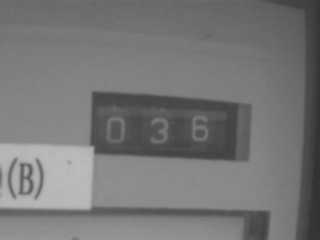
\includegraphics{gaussian.eps}
  \caption{$3\times 3$近似高斯模板}
  \label{fig:gaussian}
\end{figure}

%直接计算模板较大的高斯滤波非常耗时。为了减少计算时间。由式\eqref{eq:gauss1}和式\eqref{eq:gauss2}可得$g(x,y)=g(x)g(y)$,说明$x$和$y$方向的高斯滤波互不影响。利用这一点,可以将二维的高斯滤波器分解为两个一维的高斯滤波器,分别在$x$和$y$方向进行滤波,从而减少运算量。
% \begin{equation}
%   \label{eq:sep}
%   g(x,y)=g(x)g(y)
% \end{equation}
% 式\eqref{eq:sep}说明二维高斯函数可以用两个一维高斯函数的乘积表示,

% \begin{enumerate}[(1)]
% \item 离模板中心越远的点,其权值逐渐减小到零。
% \item 总权值集中在$2\sigma$的范围内,故用标准差$\sigma$决定邻域的范围。
% \item 多个高斯滤波可以合并为一个高斯滤波过程。
% \item 对抑制高斯白噪声非常有效。
% \end{enumerate}

%加权均值模板滤波的缺基本缺陷是抑制噪声和保留边缘的矛盾。模板越大,抑制噪声的效果越好,边缘也越模糊。这是因为当模板处在两块区域的边缘时,由于两块区域的灰度差别很大,取加权平均值导致边缘处的灰度差别变小,不利于后续的边缘检测。即用模板中心权值较大的高斯滤波模板,边缘也有一定的失真。为了做到既能减少噪声,又能保持边缘,可以采用中值滤波。中值滤波就是用模板下所有像素灰度的中值代替原像素值。由于只需知道第$\frac{1}{2}(n-1)$大的像素值,不需要知道其他像素值的相对大小,可以巧妙地改造快速排序算法求出快速地求出中值。选取数组中的某个值,如果将分割点和$\frac{1}{2}(n-1)$比较,发现当分割点小于$\frac{1}{2}(n-1)$,说明中值包含在较大的数组中,当分割点大于$\frac{1}{2}(n-1)$时,说明中值包含在较小的数组中。这时只需对包含中值的数组递归地采用上述分割方法。

\section{边缘检测}\label{sec:edge}

边缘是分割图像的一个重要特征。在灰度图像中,边缘表现为灰度有突然变化的区域\upcite{imgproc}。因此,边缘检测的经典算法是用每个像素所在邻域内的灰度变化确定边缘,而邻域内的灰度变化可以用邻域的导数刻画。这种利用利用邻域内的导数检测边缘,称为边缘检测局部算子法\upcite{imgproc}。

% \subsection{一维信号边缘检测}\label{sec:edge1d}

% 首先讨论一维信号的边缘检测算子,这不仅直观,也很容易推广到二维图像的边缘检测算子。而且一维信号的边缘检测算子也有实际用途,如用一维信号的边缘检测算子找出灰度直方图的波峰波谷。一维信号$f(x)$在邻域内的变化率用导数刻画:
% \begin{equation}
%   \label{eq:diff}
%   \frac{\mathrm{d}f}{\mathrm{d}x}=\lim_{\Delta x\to 0}\frac{f(x+\Delta x)-f(x)}{\Delta x}
% \end{equation}
% 连续信号$f(x)$无法直接观测,只能观测到间隔为1的离散信号$f(i)$,所以用差分$f'(i)=f(i+1)-f(i)$估计$f'(x)$。一阶差分相当于将模板$M'=[-1,1]$应用到一维信号中。模板$M'$的中心为左边的点。同理可得,$f(x)$的二阶导数可以用$f(i)$的二阶差分近似,相当于对$f(i)$应用模板$M''=[1,-2,1]$进行运算。

% 上述模板运算只利用了$i$和$i+1$处的值,和$i-1$没有关系。为了对称地利用$i$处的邻域,采用导数的对称的定义。
% \begin{equation}
%   \label{eq:diff2}
%   \frac{\mathrm{d}f}{\mathrm{d}x}=\lim_{\Delta x\to 0}\frac{f(x+\Delta x)-f(x-\Delta x)}{2\Delta x}
% \end{equation}
% 同样取$\Delta x=1$,得到一阶导数的近似值对应的模板为$M'_2=\frac{1}{2}[-1,0,1]$,二阶导数的近似值对应的模板为$M'_2=\frac{1}{2}[-1,-1,1,1]$。按照边缘处的一阶和二阶导数值分类,边缘可以分为阶跃形边缘、屋脊状边缘和斜坡形边缘。在阶跃形边缘处,一阶导数在此处存在一个脉冲,二阶导数在此处存在一个过零点。在屋脊状边缘处,一阶导数在此处存在阶跃,二阶导数在此处存在一个脉冲。在斜坡行边缘处,一阶导数在此处存在极值。如果发现导数存在这些特征,说明检测到边缘。

%\subsection{二维图像边缘检测}\label{sec:edge2d}

图像$f(x,y)$可能在任意方向均存在导数。其中两个特殊的方向导数分别为沿着$x$和$y$轴方向的两个导数$f_x$和$f_y$,其他方向的导数都可以表示为这两个方向导数的线性组合\upcite{calculus}。如果将$y$视为参量,则$f_x$可以视为以$x$为变量的一元函数,可以将模板$M'_2=[-1,0,1]$应用于$f(x,y)$求出该导数的近似值\upcite{compvision}。然而,由于图像含有噪声,而且边缘不一定沿$x$方向,因此应该将模板应用于像素本身及其上下两个相邻像素,求出三个近似值,再求出这三个近似值的平均值作为该处$f_x$的估计值\upcite{machvision}。这个计算过程相当于将如图\ref{fig:prewitt_x}所示的模板应用于图像$f(x,y)$。同理可得计算$f_y$的模板,如图\ref{fig:prewitt_y}所示。
\begin{figure}[!h]
  \centering
  \subfloat[x方向]{\label{fig:prewitt_x}\includegraphics{prewitt_x.eps}}\hspace{1cm}
  \subfloat[y方向]{\label{fig:prewitt_y}\includegraphics{prewitt_y.eps}}
  \caption{Prewitt算子}
\end{figure}
一种类似的算子是Sobel算子,如图\ref{fig:sobel}所示,它对中间一行运算的权值是上下两行的权值的两倍。
\begin{figure}[!h]
  \centering
  \subfloat[x方向]{\includegraphics{sobel_x.eps}}\hspace{1cm}
  \subfloat[y方向]{\includegraphics{sobel_y.eps}}
  \caption{Sobel算子}
  \label{fig:sobel}
\end{figure}

根据二元函数微分学,二维图像$f(x,y)$沿\emph{梯度}方向灰度变化最大\upcite{calculus}。图像的梯度定义为向量$\nabla f=(f_x,f_y)$,梯度的幅值为$|\nabla f|=\sqrt{f_x^2+f_y^2}$,方向为$0=\arctan\left(\frac{f_y}{f_x}\right)$。为了减少计算量,梯度幅值一般简化为计算$\frac{1}{2}(f_x^2+f_y^2)$或$\max(|f_x|,|f_y|)$或$|f_x|+|f_y|$。另一种简化计算梯度的方法是利用与标准行列方向偏离45度的两个交叉的差分作为方向导数\upcite{imgproc}。这两个方向导数在$(i,j)$处的估计值为$f(i+1,j+1)-f(i,j)$和$f(i,j+1)-f(i,j+1)$。这两个差分运算可以用图\ref{fig:robert}所示的模板表示,称为Roberts算子。用上述算子求出梯度和幅值后,追踪具有高幅值的点,或追踪幅度极值点,可以得到边缘。
\begin{figure}[!h]
  \centering
  \subfloat{\includegraphics{robert_x.eps}}\hspace{1cm}
  \subfloat{\includegraphics{robert_y.eps}}
  \caption{Robert算子}
  \label{fig:robert}
\end{figure}

上述边缘算子的基本缺陷就是检测精度和抗噪声能力不能兼顾\upcite{imgproc}。由于图像的边缘和噪声均为灰度急剧变化的部分,简单的梯度运算会将噪声误认为边缘。Canny应用严格的数学方法分析边缘检测的缺陷,并提出平衡检测精度和抗噪声能力的方法。Canny给出了评价边缘检测的三个准则\upcite{machmeter}:
\begin{asparaenum}[(1)]
\item 信噪比准则:信噪比越大,边缘质量越高。
\item  定位精度准则,即检测出的边缘点尽量靠近实际边缘。
\item 单边缘响应准则:即单个边缘只产生一个响应,虚假边缘响应得到最大抑制。
\end{asparaenum}

为满足上述准则,Canny利用最优化方法,得到了最佳边缘模板。Canny针对一维边缘,推导出的最优边缘检测算子与高斯函数的导数类似。在实际应用中,为了减少计算量,可以用高斯滤波后再用Sobel算子求出方向导数的幅度和方向,用于近似计算Canny的最优边缘检测算子\upcite{opencvref}。

此时得到原始图像的梯度图像。梯度较大处都是边缘的候选点。但一个真实的边缘点附近往往有许多虚假的边缘响应,在图像中表现为一条较粗的边缘。为了细化边缘,在邻域内的多个边缘响应点只用保留一个。通过判断候选点是否为其梯度方向上的邻域的极大值判定该点是否为边缘点\upcite{opencvref}。%具体做法是,对某个候选点,在其梯度方向上找出一个邻点,要求该邻点和候选点的连线与梯度方向相差不到45度。然后再其梯度的反方向上满足同样要求的邻点。比较候选点和这两个邻点的梯度幅值,如果候选点的梯度幅值高于两个邻点,则保留该候选点,否则删除该候选点。
这一过程称为\emph{非极大值抑制}。
% \begin{algorithm}[H]
%   \caption{非极大值抑制}
% \label{alg:nms}
% \begin{algorithmic}
%   \REQUIRE $\textrm{梯度幅值图像}M\textrm{和梯度方向图像}D$
% \ENSURE $\textrm{边缘细化的梯度图像}N$
% \FOR {$i\gets 0$ \TO $\max(i)$}
% \FOR {$j\gets 0$ \TO $\max(j)$}
% \STATE $N_1[4]\gets\{(1,0),(1,1),(0,1),(-1,1)\}$
% \STATE $N_2[4]\gets\{(-1,0),(-1,-1),(0,-1),(1,-1)\}$
% \STATE $d\gets D(i,j) \mod \frac{\pi}{4}$
% \STATE $(u_1,v_1)\gets (i,j)+N_1[d]$
% \STATE $(u_2,v_2)\gets (i,j)+N_2[d]$
% \IF {$M(i,j) > M(u_1,v_1)$ \AND $(M(i,j) > M(u_2,v_2)$}
% \STATE $N(i,j)\gets M(i,j)$
% \ELSE
% \STATE $N(i,j)\gets 0$
% \ENDIF
% \ENDFOR
% \ENDFOR
% \end{algorithmic}
% \end{algorithm}

过极大值抑制后,边缘仅为单像素宽。然而这些边缘仍然存在虚假边缘响应点。使用双阈值的方法提高边缘质量。选取高低两个阈值。在梯度图像中找出幅度高出高阈值的点\upcite{opencvref}。然后将这些邻点作为新的起点,再找出它们周围高于低阈值的邻点。

\section{图像分割}

图像分割就是将图像划分成多个区域,这些区域内的特征表现相似,而不同区域间特征显著不同\upcite{imgproc}。常见的特征有灰度、色彩、纹理和几何形状\upcite{machvision}。图像分割的有两个目的。第一个目的是分离目标和背景,为图像识别奠定基础。第二个目的将像素组织成更高级的单元,进而从区域的角度而不是像素的角度更好地分析图像\upcite{compvision}。
目前没有一种通用的分割方法,适用于各个领域,需要根据具体情况选择合适的分割算法。

\subsection{阈值分割}

阈值分割假定不同的区域的灰度值有显著差异,区域内的像素值在一个较小范围内浮动。许多图像满足这一假设。根据这一假设,找出各个区域的灰度区间,找出区间内的像素,即可完成分割。不同灰度区间的分界点称为\emph{阈值}。有多种方法可以选取阈值。最简单的情况是选取单阈值,将图像分割为低于阈值的部分和高于阈值的部分。还有双阈值的情况,即选取一个较高的阈值和较低的阈值,将图像分割为处于高低阈值之间的区域,和在高低阈值之外的区域。阈值可以由用户指定,但为了自动处理和识别图像,应根据图像的特点计算合适的阈值\upcite{compvision}。

计算阈值的基本依据是直方图。如果能估计待分割区域的占整个图像的百分比$p$,则找出一个阈值,使低于(高于)阈值部分的灰度出现概率为$p$即可完成分割\upcite{vcimg}。如果区域的百分比不能确定,可以根据直方图的波峰和波谷计算阈值。直方图的波峰对应区域内像素的平均灰度,波谷对应区域边界的灰度,因此选取两个波峰之间的波谷对应的灰度作为阈值\upcite{otsu}。%如果两个区域的灰度有重叠,直方图的波峰波谷不明显,或区域之间的面积比例悬殊,该方法的分割效果不理想。

自动确定阈值的另一种常见方法是Otsu算法\upcite{otsu}。该算法假定目标和背景区域分别为黑白两种像素,或图像的直方图呈现双模式分布。设$P(i)$表示灰度$i$出现的概率,$t$为候选阈值,$\mu_1(t)$和$\sigma_1^2)$分别表示低于阈值$t$的区域的均值和方差,$\mu_2(t)$和$\sigma_2^2(t)$分别表示高于阈值$t$的区域的均值和方差,$q_1(t)$和$q_2(t)$分别是两个区域的灰度百分比。则组内方差$\sigma_W^2(t)$的定义为:
\begin{equation}
  \label{eq:sigw}
  \sigma_2^2(t)=q_1(t)\sigma_1^2(t)+q_2(t)\sigma_2^2(t)
\end{equation}

其中
\begin{equation}
  \label{eq:musig}
  \begin{aligned}
    q_1(t) &= \sum_{i=0}^tP(i) \quad & q_2(t) &= \sum_{i=t+1}^{L-1}P(i) \\
    \mu_1(t) &= \sum_{i=0}^t\frac{iP(i)}{q_1(t)} \quad & \mu_2(t) &= \sum_{i=t+1}^{L-1}\frac{iP(i)}{q_2(t)} \\
    \sigma_1(t) &= \sum_{i=1}^t\frac{[i-\mu_1(t)]^2}{q_1(t)} \quad & \sigma_2(t) &= \sum_{i=t+1}^{L-1}\frac{[i-\mu_2(t)]^2}{q_2(t)}
  \end{aligned}
\end{equation}

Otsu算法找出使组内方差最小$\sigma_W^2(t)$的$t$作为阈值。如果直接按式\ref{eq:sigw}计算所有可能的$t$值,则对每个$t$值都需要分别求出两个区域的均值和方差,计算效率低下。可以用总方差和组内方差的关系简化计算\upcite{opencvref}。总方差的定义为:
\begin{equation}
  \label{eq:var}
  \sigma^2=\sum_{i=1}^{L-1}(i-\mu)^2P(i)
\end{equation}
由\eqref{eq:sigw}和\eqref{eq:var}可得:
\begin{equation}\begin{split}
  \label{eq:sigrel}
  \sigma^2 =&[q_1(t)\sigma_1^2(t)+q_2(t)\sigma_2^2(t)] \\
  &  +\{q_1(t)[\mu_1(t)-\mu]^2+q_2(t)[\mu_2(t)-\mu]^2\}
\end{split}\end{equation}
式\eqref{eq:sigrel}的第一项是组内方差$\sigma_W^2$,第二项是组间方差$\sigma_B^2$。由于总体方差和$t$无关,故组内方差最小时,最间方差最大,故通过计算每个$t$值的组内方差找出阈值\upcite{compvision}。总均值$\mu$和两个区域的均值$\mu_1(t),\mu_2(t)$和百分比$q_1(t),q_2(t)$的关系为:
\begin{equation}
  \label{eq:sigma}
  \mu=q_1(t)\mu_2(t)+q_2(t)\mu_2(t)
\end{equation}
将式\eqref{eq:sigma}代入式\eqref{eq:sigrel},消去$\mu$,组间方差可以简化为:
\begin{equation}
  \label{eq:sigb}
  \sigma_B^2(t)=q_1(t)q_2(t)[\mu_1(t)-\mu_2(t)]^2
\end{equation}
找出使$\sigma_B^2(t)$最大的$t$值,作为Otsu算法的阈值。%用公式表示为:
% \begin{equation}
%   \label{eq:otsu}
%   t^{*}=\arg\max_{0\leqslant t\leqslant L-1}\sigma_B^2(t)
% \end{equation}

如果图像的背景亮度不均匀,则全局阈值分割效果不理想,因为不同的区域平均亮度有差别,对平均亮度不同的区域使用相同的阈值,导致部分像素被错分。这种情况可以使用局部阈值法。局部阈值法对每个像素的邻域均计算一个局部阈值,将邻域中心像素和局部阈值比较,确定所在区域\upcite{opencvref}。局部阈值法的缺点是计算量比全局阈值法大,容易在目标区域内形成裂痕或空洞,而且邻域的大小严重影响分割效果\upcite{meter1}。因此应根据图像的特点选择邻域大小和局部阈值的计算方式。


% 式\eqref{eq:sigb}的四项$q_t(t),q_2(t),\mu_1(t),\mu_2(t)$可以用递推公式计算,计算方式为:
% \begin{subequations}
%   \begin{align}
%     q_1(t+1) &= q_1(t)+P(t+1) \\
%     q_2(t+1) &= 1-q_1(t) \\
%     \mu_1(t+1) &= \frac{q_1(t)\mu_1(t)+(t+1)P(t+1)}{q_1(t+1)} \\
%     \mu_2(t+1) &= \frac{\mu-q_1(t+1)\mu_1(t+1)}{1-q_1(t+1)}
%   \end{align}
% \end{subequations}

\subsection{边缘分割}

边缘分割利用图像的边缘分割图像。用\ref{sec:edge}节所述的边缘检测算子找出边缘点后,再将边缘点连成轮廓线,分割轮廓线两边的区域\upcite{compvision}。边缘检测算子容易产生虚假的边缘又丢失部分边缘,从而产生边缘缺口\upcite{machvision}。如果轮廓线的曲线类型已知,如直线或圆等,则用哈夫变换对于有缺口的边缘也能产生较好的分界线。哈夫变换的基本思想就是借助带参曲线方程,先将图像空间的点变换成参数空间的曲线集合,再将参数空间的曲线交点变换成图像空间的曲线集合。下面以边缘直线检测为例介绍哈夫变换。

首先要定义带参直线方程。直线方程通常的定义为:
\begin{equation}
\label{eq:scope}
  y=kx+b
\end{equation}
式\eqref{eq:scope}不能表示和$x$轴平行的直线,这是由于参数$k$只能取有限值。更好的参数向量是原点到直线的垂直向量,用向量的长度$\rho$和倾斜角$\theta$表示\upcite{machvision}。带参数$\rho$和$\theta$的直线方程为:
\begin{equation}
  \label{eq:polar}
  \rho=x\cos\theta+y\sin\theta
\end{equation}
式\eqref{eq:polar}可以表示任意方向的直线,因此作为带参直线方程。对于给定的$(x,y)$,参数方程可以看作参数空间的一条正弦曲线。由于正弦函数具有周期性,$\theta$只用取$[0,2\pi)$范围内的值。设图像中有$n$个点$(x_1,y_1),(x_2,y_2),\cdots,(x_n,y_n)$。这些点的方程分别为:
\begin{equation}
\label{eq:func}
  \rho=x_i\cos\theta+y_i\sin\theta,\quad i=1,2,\cdots,n
\end{equation}
式\eqref{eq:func}说明这$n$个点对应参数空间的$n$条正弦曲线。若这些点共线,则存在一条参数为$\rho_0$和$\theta_0$的直线$\rho_0=x\cos\theta_0+y\sin\theta_0$。将$(x_i,y_i)$代入直线方程,不难看出$(\rho,\theta)$为式\eqref{eq:func}表示的一组曲线的交点。故在参数空间中找出交点,即可找出图像的直线。

从曲线的方程求出交点非常困难,所以我们将曲线“画”出曲线的图像。而要画出曲线图像,需要对参数空间进行离散化。分别指定$\rho$和$\theta$的很小的量化间隔$\Delta\rho$和$\Delta\theta$,得到$\rho$和$\theta$的一组离散值。对每对离散的$(\rho,\theta)$指定一个像素值$A(\rho,\theta)$。这些像素构成一个二维的\emph{累加器数组},其初值均为零\upcite{machvision}。对$\theta$的所有离散值$\theta'$,计算对应的$\rho$值。然后量化$\rho$,即找出最接近$\rho$的离散值$\rho'$。然后将累加器数组内位于$(\theta',\rho')$处的值加1,表示曲线通过该像素。显然,累加器数组的值表示通过该处的曲线数,对应于边缘图像共线的点数。累加器数组的峰值是曲线的多重交点,对应边缘图像中共点最多的直线,即为检测出的直线。

\section{二值图像分析}

图像分割后的结果一般是二值图像,其中目标像素值设为1。背景像素值设为0。在文档扫描和工业机器视觉系统中,计算机系统都是以二值图像作为识别的对象。二值图像算法的应用场合十分广泛,例如目标计数、定位和识别等\upcite{machvision}。

\subsection{连通成分标记}\label{sec:comp}

\emph{连通成分}指具有相同的灰度且其中任意像素都有相邻像素的像素集合。连通成分标记就是用不同的标号区分不同的连通成分,每个连通成分的像素值设定为其所在的连通成分的标号。标记连通成分有两种基本算法:\emph{递归搜索算法}和\emph{逐行扫描算法}\upcite{machvision}。

递归搜索算法的基本思想是将某个具有最大灰度的像素作为种子像素,将其像素值设定为连通成分的标号\upcite{machvision}。再从其相邻的像素中找出未标记且值为1的像素,将这些像素作为新的种子像素,递归地施行上述方法,直到标记完连通成分的所有像素。然后找出另一连通成分的种子像素,施行同样的方法,直至标记出所有的连通成分。%设$B$表示二值图像,$LB$表示连通成分的标记图像,$LB(i,j)$的初值为0,则算法如\ref{alg:comp}所示。
% \begin{algorithm}[H]
%   \caption{标记二值图像的连通成分}
%   \label{alg:comp}
%   \begin{algorithmic}
%     \REQUIRE $\textrm{二值图像}B$
%     \ENSURE $\textrm{连通成分标记}LB$
%     \STATE $label\gets 0$
%     \FOR{$i\gets 0$ \TO $M-1$}
%     \FOR{$j\gets 0$ \TO $N-1$}
%     \IF{$B(i,j)=1$ \AND $LB(i,j)=0$}
%     \STATE $label\gets label+1$
%     \STATE $\search(i,j,label)$
%     \ENDIF
%     \ENDFOR
%     \ENDFOR
%     \STATE $\textbf{procedure}\ \search(i,j,label)$
%     \STATE $LB(i,j)\gets label$
%     \STATE $N\gets \neighbours(i,j)$
%     \FOR{$(i',j')\in N$}
%     \IF{$B(i',j')=1$ \AND $LB(i',j')=0$}
%     \STATE $\search(i',j',label)$
%     \ENDIF
%     \ENDFOR
%   \end{algorithmic}
% \end{algorithm}

在递归扫描算法中,每扫描一个像素就要做一次递归。数字图像的像素点很多,递归深度非常大,因此算法的时间和空间开销非常大。有人提出了逐行扫描算法\upcite{machvision},只需扫描图像两次。该算法扫描图像时,找出未标记的像素作为种子像素,设定其临时标号,将种子像素的临时标号传播到后续像素。由于种子像素的标号只能向右下转播,故其左下方也可能存在另一个种子像素\footnote{种子像素$P$的右上方也有可能存在种子像素$Q$。在这种情况下,我们将像素$Q$当作“当前”像素,则$P$仍然是“左下方”的像素。左上方的种子像素和“当前”种子像素不可能在同一个连通成分内,否则左上方的种子像素会将标号传播到“当前”种子像素,此时“当前”像素不是种子像素。所以只用考虑合并“当前”像素及其左下方像素的传播区域。}两个种子像素的标号可能传播到同一区域。如果出现这种情况,说明两个种子像素传播的区域在同一个连通成分内,说明这两个临时标号其实标记了同一个连通成分,是两个等价的标号。为了确保同一连通成分内只有一个标号,需要再次扫描图像,将临时标号用其等价标号代替。该算法需要记录标号之间的等价关系,在发现两个标号等价需要更新等价关系。\emph{并查集}特别适合记录、更新和查找等价关系\upcite{alg}。

并查集是一种存储不相交的集合的数据结构\upcite{alg}。它有三个基本操作$\make,\find$和$\union$。其中$\make(x)$创建一个仅包含元素$x$的集合,$\find(x)$查找元素$x$所在的集合,$\union(x,y)$合并元素$x$和$y$所在的集合。并查集一般用树的集合表示。树中的每个结点表示集合的一个元素。每个结点只指向其结节点,根节点代表整个集合。%实现$\find(x)$操作的一种简单的方法是从结点$x$开始,找到其父节点,再找到父结点的父结点……直到找到根结点,将根结点作为集合的代表。实现$\union(x,y)$操作的一种简单的方法是用$\find(x)$和$\find(y)$操作找到$x$和$y$的根结点,然后将$x$的根结点指向$y$的根结点,反之也行。

\subsection{数学形态学}\label{sec:morph}

\emph{数学形态学}是建立在集合代数理论上,分析几何形状和结构的数学的学科,最初用于岩石结构分析。形态学的主要用途是获取并改变物体的拓扑结构\upcite{machmeter}。通过将结构元作用于几何形状,可以得到物体更本质的形态。进入八十年代,数学形态学被引入机器视觉领域后,人们对其进行深入的研究和广泛的应用。至今理论上已趋于完备,应用领域上不断拓展,应用到平滑滤波、边缘检测、特征提取、形状描述、模型构造等图像处理的方方面面\upcite{machmeter}。

\emph{二值形态学}是数学形态学最简单的情况\upcite{machvision},它具有运算简单、效果显著的特点。二值形态学运算是用一个较小的二值图像在图像上进行运算。这个较小的图像称为\emph{结构元}。在定义形态学运算前,先定义\emph{平移}运算。设$A$表示几何形状的像素坐标集合,则有序对$b$对$A$平移运算定义为对$A$的每个坐标加上有序对$b$,用公式表示为\upcite{machvision}:
\begin{equation}
  \label{eq:shift}
  A_b=\{a+b|a\in A\}
\end{equation}

二值形态学最基本的运算是\emph{膨胀}和\emph{腐蚀}。设二值图像值为1的像素的坐标集合为$A$,结构元中值为1的像素坐标集合为$B$,则定义$A$关于$B$的膨胀运算为用$B$内所有坐标对$A$进行平移,记为$A\oplus B$,如下所示:
\begin{equation}
  \label{eq:dilate}
  A\oplus B=\bigcup_{b\in B}A_b=\{a+b|a\in A,b\in B\}
\end{equation}

式\eqref{eq:dilate}是从集合的角度定义膨胀运算,也可以从图像的角度直观地定义膨胀运算。从图像上看,膨胀运算相当于结构元在图像上移动,让结构元中心与像素重合,当遇到值为1的像素时,将结构元上的值和结构元下对应位置的像素做“或”运算\upcite{compvision}。图\ref{fig:binary}和图\ref{fig:struct}分别是二值图像和结构元,图\ref{fig:dilate}是两者的膨胀运算结果。从图上看出,膨胀运算使形状的区域扩大。

\begin{figure}[h]
  \centering
  \subfloat[二值图像]{\label{fig:binary}\includegraphics{binary.eps}}\hspace{1cm}
    \subfloat[结构元]{\label{fig:struct}\includegraphics{struct.eps}}\\
    \subfloat[膨胀运算]{\label{fig:dilate}\includegraphics{dilate.eps}}\hspace{1cm}
    \subfloat[腐蚀运算]{\label{fig:erode}\includegraphics{erode.eps}}\\
  \subfloat[开运算]{\label{fig:open}\includegraphics{open.eps}}\hspace{1cm}
  \subfloat[闭运算]{\label{fig:close}\includegraphics{close.eps}}
  \caption{形态学运算}
\end{figure}

定义$A$关于$B$的腐蚀运算为,用$B$中所有坐标对$A$进行平移运算后,找出仍然在$A$中的坐标,将这些坐标组成一个集合\upcite{machvision}。腐蚀运算记为$A\ominus B$,用公式表示为:
\begin{equation}
  \label{eq:erode}
  A\ominus B=\{a|(a+b)\in A\quad\textrm{for}\ a\in A,b\in B\}=\bigcap_{b\in B}A_b
\end{equation}

从图像上看,腐蚀运算也是将结构元中心在图像上移动,只有当结构元上值为1的位置覆盖的像素值均为1时,才将结构元和其覆盖的像素进行“或”运算\upcite{compvision}。腐蚀运算的结果如图\ref{fig:erode}所示。从图上发现,腐蚀运算使区域缩小。

在腐蚀和膨胀运算的基础上定义开运算和闭运算。开运算就是腐蚀再膨胀,记为$A\circ B=(A\ominus B)\oplus B$。闭运算就是膨胀再腐蚀\upcite{compvision}。图\ref{fig:open}和图\ref{fig:close}分别是开运算和闭运算的结果。


数学形态学的基本操作有许多应用。在二值图像中,如果某个区域内部有小孔,可以用尺寸与小孔相同的模板进行闭运算以填充小孔\upcite{compvision}。如果两个不同的区域中间有细小的线段连接,为了消除这些线段,可以使用开运算。在工业检测中,形态学运算可用于检测零件的缺陷。

\section{本章小结}

本章的主要内容是介绍数字图像处理的基本理论。主要介绍了
%%% Local Variables: 
%%% mode: latex
%%% TeX-master: "thesis"
%%% End: 
